
%=+=+=+=+=+=+=+=+=+=+=+=+=+=+=+=+=+=+=+=+=+=+=+=+=+=+=+=+=+=+=+=+=+=+=+=+=+=+=+=
%             _             _
%            | |           | |
%  _ __ ___  | |__    ___  | | ___   ___   _ __       ___   ___   _ __ ___ 
% | '_ ` _ \ | '_ \  / _ \ | |/ __| / _ \ | '_ \     / __| / _ \ | '_ ` _ \ 
% | | | | | || | | || (_) || |\__ \| (_) || | | | _ | (__ | (_) || | | | | | 
% |_| |_| |_||_| |_| \___/ |_||___/ \___/ |_| |_|(_) \___| \___/ |_| |_| |_| 
%
% Author: Mark H. Olson
% Website: https://mholson.com
% Github: https://github.com/mholson
%
% Created: 2015-07-31
%
% Enter Text here
%=+=+=+=+=+=+=+=+=+=+=+=+=+=+=+=+=+=+=+=+=+=+=+=+=+=+=+=+=+=+=+=+=+=+=+=+=+=+=+=




%=-=-=-=-=-=-=-=-=-=-=-=-=-=-=-=-=-=-=-=-=-=-=-=-=-=-=-=-=-=-=-=-=-=-=-=-=-=-=-=
% PREAMBLE :: main.tex 
%=-=-=-=-=-=-=-=-=-=-=-=-=-=-=-=-=-=-=-=-=-=-=-=-=-=-=-=-=-=-=-=-=-=-=-=-=-=-=-=
%
% > > >	The following beamer class options are available
%?		aspectratio			= 169
%?		sectionpages
%
% > > > The following sthlmnord package options are available
%?		mode				= dark (default)
%?							= light
%=-=-=-=-=-=-=-=-=-=-=-=-=-=-=-=-=-=-=-=-=-=-=-=-=-=-=-=-=-=-=-=-=-=-=-=-=-=-=-=

\documentclass[aspectratio=169, sectionpages]{beamer}
\usetheme[mode=light]{sthlmnord}

% > > > CTAN Packages
%		the subfiles package is being used to compile individual slides
%		using the main tex file.  Individual slides can then be included
%		into multiple slide decks.
\usepackage{subfiles}

% > > > Custom Packages
\usepackage{mhomath}

% > > > Generate some Lorem Ipsum placeholder text.
\usepackage{lipsum}

% > > >	Image File Paths
% 		Here you can add one or more paths to where your images are being
%		stored.  This will allow you to include only the image file 
%		name when placing it into your document.
%\graphicspath{{path1},{path2},{path3}}
\graphicspath{{./assets/}} 

\newcommand{\snord}{\cnordTen{sthlm}\cnordEight{NORD}}

% > > > Document Information
\title{sthlmNord Beamer Theme (version 3)}
\subtitle{Stockholm Inspired By Nord}
\newcommand{\course}{Fancy Courses Title Goes Here}
\newcommand{\filename}{\currfilebase}
\author{markolsonse}
\institute{Some School in Stockholm}
\date{\today}
%\titlegraphic{nordtitlelogodark}
\titlegraphic{nordtitlelogolight}

% > > > pdf customizations via hyperref (pkg installed by beamer)
\hypersetup{
colorlinks=true,
% You might want to disable color links for you final draft.
%colorlinks=false,
linkcolor={nordNine},
citecolor={nordNine},
urlcolor={nordNine}
}

%=-=-=-=-=-=-=-=-=-=-=-=-=-=-=-=-=-=-=-=-=-=-=-=-=-=-=-=-=-=-=-=-=-=-=-=-=-=-=-=
%
%    DOCUMENT BEGINS HERE 
%
%=-=-=-=-=-=-=-=-=-=-=-=-=-=-=-=-=-=-=-=-=-=-=-=-=-=-=-=-=-=-=-=-=-=-=-=-=-=-=-=
\begin{document}

%=-=-=-=-=-=-=-=-=-=-=-=-=-=-=-=-=-=-=-=-=-=-=-=-=-=-=-=-=-=-=-=-=-=-=-=-=-=-=-=
%   TITLE START   -=-=-=-=-=-=-=-=-=-=-=-=-=-=-=-=-=-=-=-=-=-=-=-=-=-=-=-=-=-=-=
\titlepage
%   TITLE END   --==-=-=-=-=-=-=-=-=-=-=-=-=-=-=-=-=-=-=-=-=-=-=-=-=-=-=-=-=-=-=
%=-=-=-=-=-=-=-=-=-=-=-=-=-=-=-=-=-=-=-=-=-=-=-=-=-=-=-=-=-=-=-=-=-=-=-=-=-=-=-=

%=-=-=-=-=-=-=-=-=-=-=-=-=-=-=-=-=-=-=-=-=-=-=-=-=-=-=-=-=-=-=-=-=-=-=-=-=-=-=-=
%   FRAME START   -=-=-=-=-=-=-=-=-=-=-=-=-=-=-=-=-=-=-=-=-=-=-=-=-=-=-=-=-=-=-=
{
\setbeamertemplate{background canvas}{\begin{tikzpicture}\node[opacity=.8,inner sep=0pt]{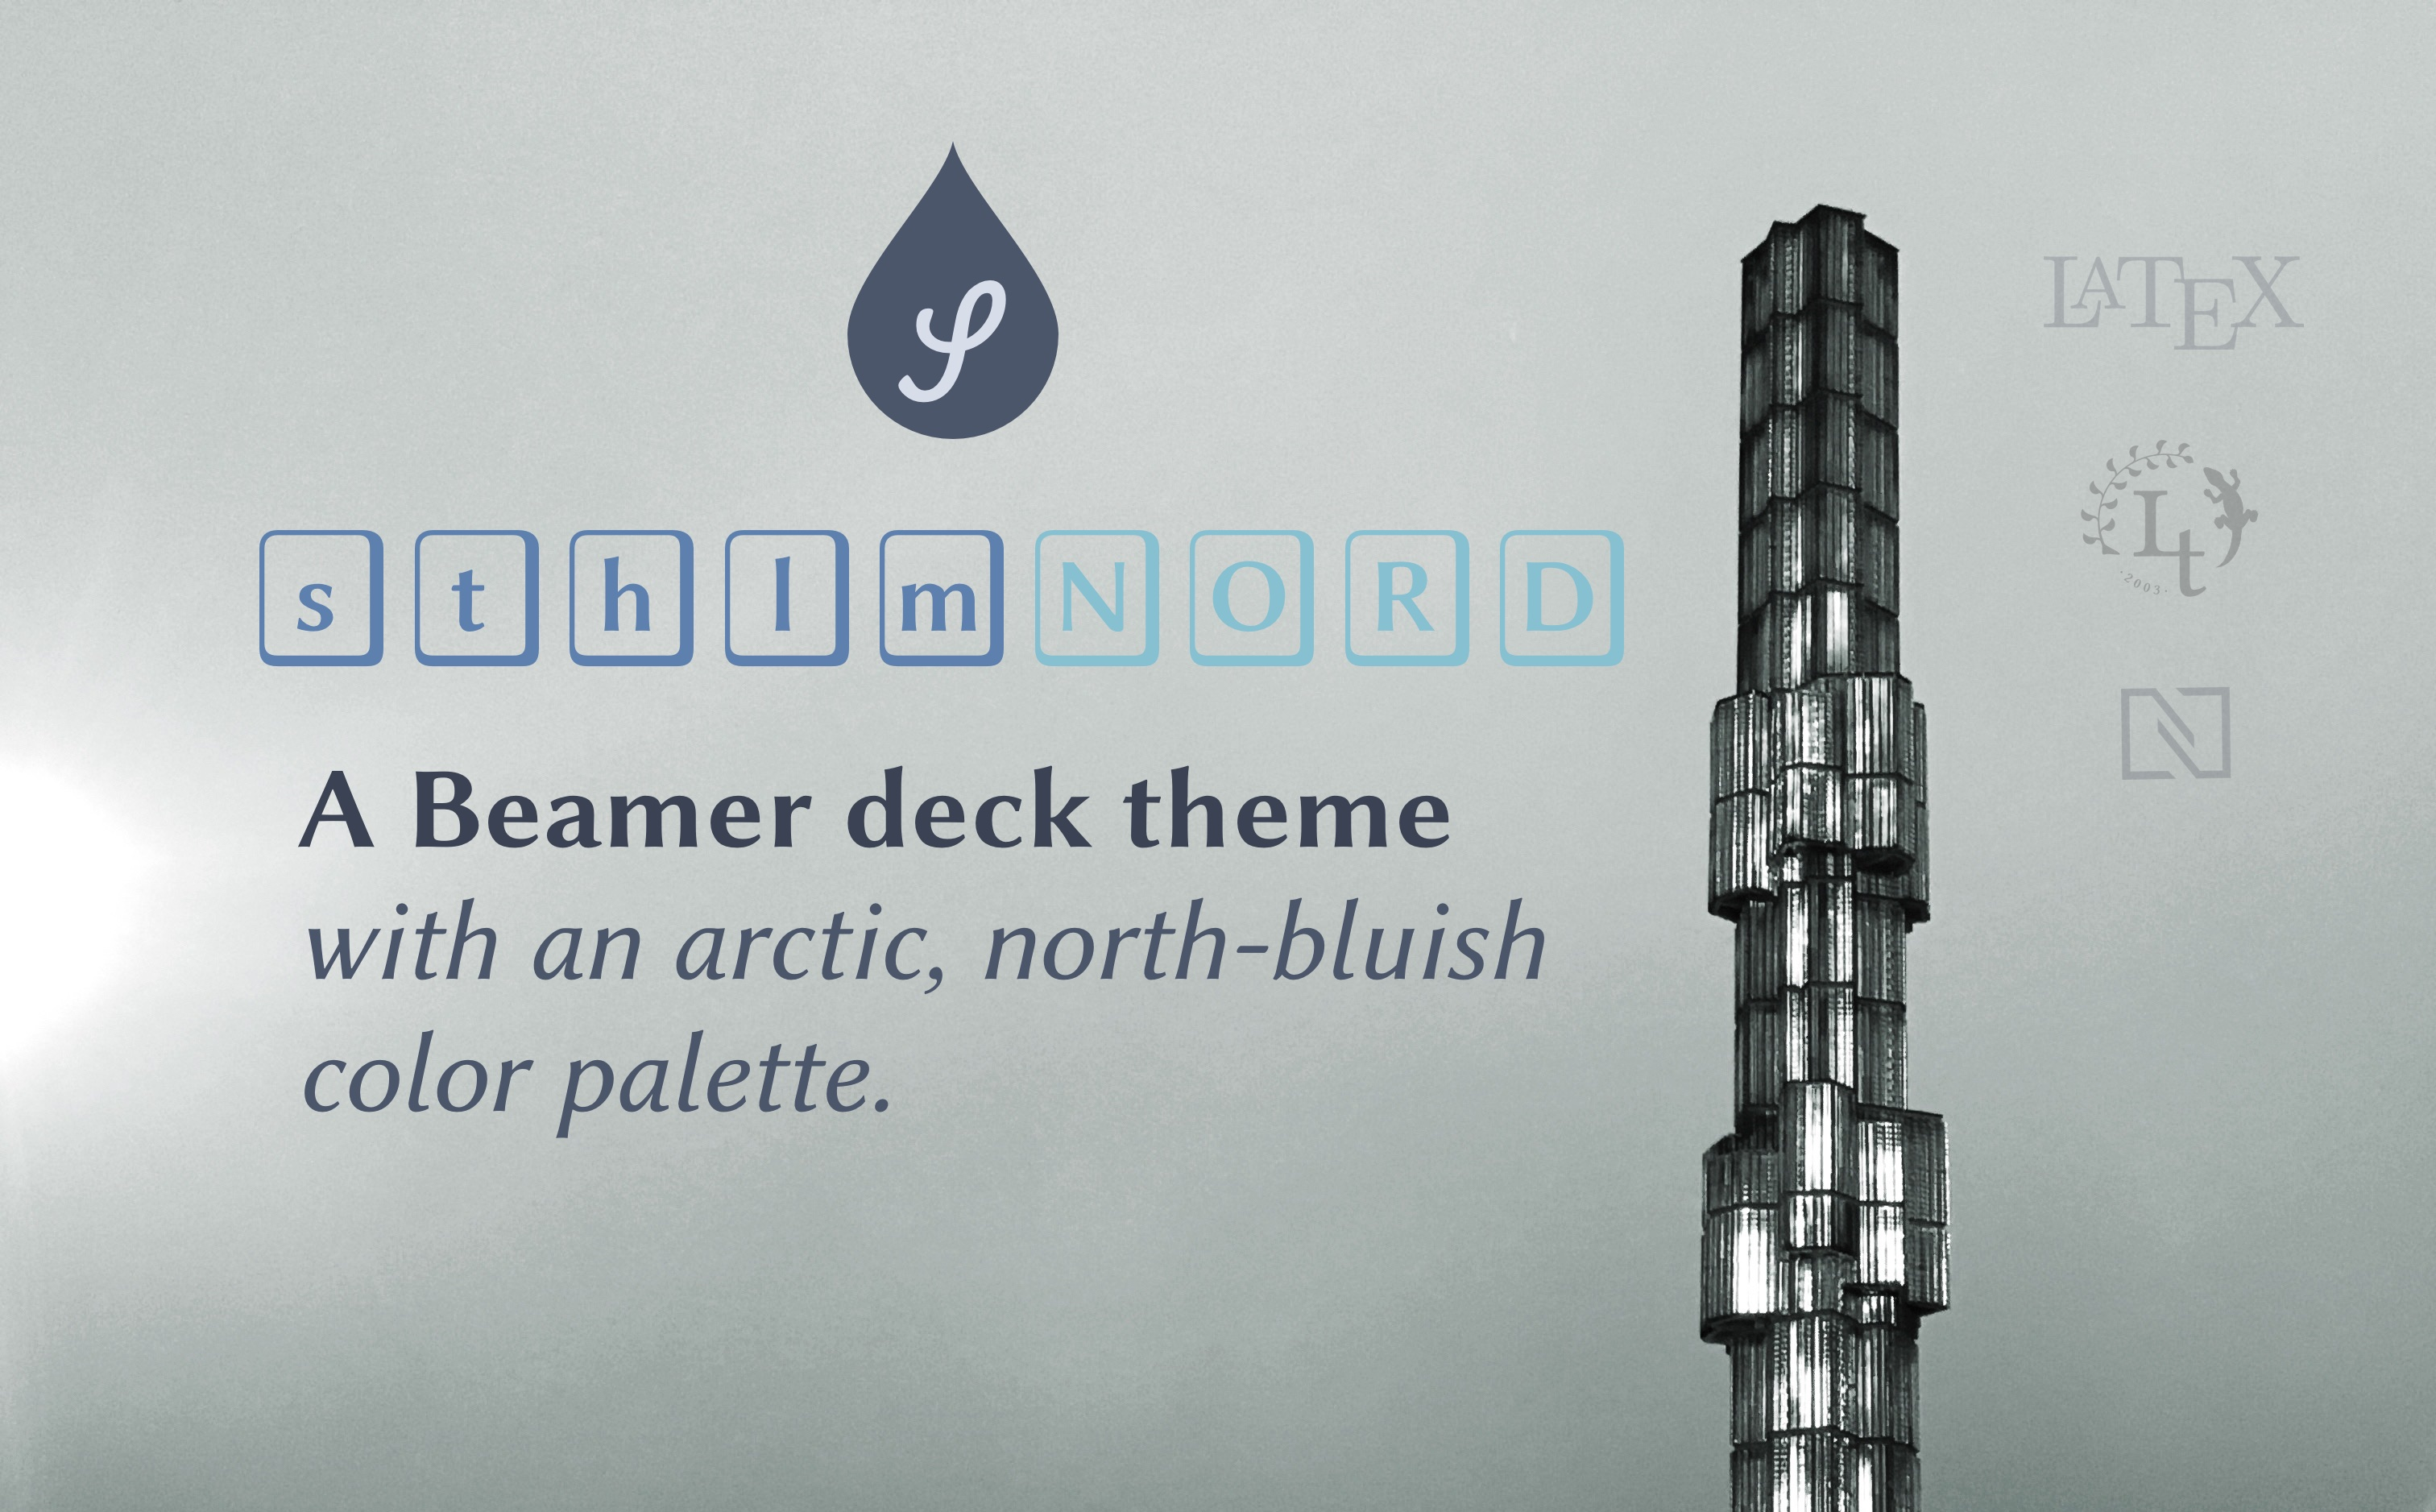
\includegraphics
		[width=\paperwidth,keepaspectratio]{nordsegel}};\end{tikzpicture}}
\begin{frame}[plain]{}

\end{frame}
}
%   FRAME END   --==-=-=-=-=-=-=-=-=-=-=-=-=-=-=-=-=-=-=-=-=-=-=-=-=-=-=-=-=-=-=
%=-=-=-=-=-=-=-=-=-=-=-=-=-=-=-=-=-=-=-=-=-=-=-=-=-=-=-=-=-=-=-=-=-=-=-=-=-=-=-=


%=-=-=-=-=-=-=-=-=-=-=-=-=-=-=-=-=-=-=-=-=-=-=-=-=-=-=-=-=-=-=-=-=-=-=-=-=-=-=-=
%   TABLE OF CONTENTS START   -=-=-=-=-=-=-=-=-=-=-=-=-=-=-=-=-=-=-=-=-=-=-=-=-=
\begin{frame}
\frametitle{Table of contents}
% > > > For longer presentations use \tableofcontents[hideallsubsections] option
%		It is also possible to manually control the entries of the table of 
% 		contents by sections.
%\tableofcontents[sections={1-10}]
%\framebreak
%\tableofcontents[sections={11-15}]
\tableofcontents
\end{frame}
%   TABLE OF CONTENTS END   -=-=-=-=-=-=-=-=-=-=-=-=-=-=-=-=-=-=-=-=-=-=-=-=-=-=
%=-=-=-=-=-=-=-=-=-=-=-=-=-=-=-=-=-=-=-=-=-=-=-=-=-=-=-=-=-=-=-=-=-=-=-=-=-=-=-=



%=-=-=-=-=-=-=-=-=-=-=-=-=-=-=-=-=-=-=-=-=-=-=-=-=-=-=-=-=-=-=-=-=-=-=-=-=-=-=-=
% SECTION 
%=-=-=-=-=-=-=-=-=-=-=-=-=-=-=-=-=-=-=-=-=-=-=-=-=-=-=-=-=-=-=-=-=-=-=-=-=-=-=-=
\section{Background Information}


%=-=-=-=-=-=-=-=-=-=-=-=-=-=-=-=-=-=-=-=-=-=-=-=-=-=-=-=-=-=-=-=-=-=-=-=-=-=-=-=
%   FRAME START   -=-=-=-=-=-=-=-=-=-=-=-=-=-=-=-=-=-=-=-=-=-=-=-=-=-=-=-=-=-=-=
\begin{frame}{Please use Metropolis Theme Instead}

Thank you for wanting to use sthlmNord version 3.

\vspace{1em}
\begin{alertblock}{Warning Label}
\cnordEleven{\textbf{You really should consider}} using the Metropolis 
theme (mTheme) instead, which has been developed \& maintained by Matthias 
Vogelgesang, as it is well tested, documented and available through CTAN. 
\end{alertblock}
\begin{center}
	\url{https://github.com/matze/mtheme}
\end{center}
\end{frame}
%   FRAME END   --==-=-=-=-=-=-=-=-=-=-=-=-=-=-=-=-=-=-=-=-=-=-=-=-=-=-=-=-=-=-=
%=-=-=-=-=-=-=-=-=-=-=-=-=-=-=-=-=-=-=-=-=-=-=-=-=-=-=-=-=-=-=-=-=-=-=-=-=-=-=-=


%=-=-=-=-=-=-=-=-=-=-=-=-=-=-=-=-=-=-=-=-=-=-=-=-=-=-=-=-=-=-=-=-=-=-=-=-=-=-=-=
%   FRAME START   -=-=-=-=-=-=-=-=-=-=-=-=-=-=-=-=-=-=-=-=-=-=-=-=-=-=-=-=-=-=-=
\begin{frame}[c,fragile]{Major Features}

	\begin{itemize}
		\item Inspired by HSRM, mTheme and Flux.
		\item Arctic Ice Studio Nord Color Theme.
		\item Libertinus fonts compiled with \XeLaTeX. 
		\item Dark (default) and Light Themes available.
	\end{itemize}
	
	\end{frame}
%   FRAME END   --==-=-=-=-=-=-=-=-=-=-=-=-=-=-=-=-=-=-=-=-=-=-=-=-=-=-=-=-=-=-=
%=-=-=-=-=-=-=-=-=-=-=-=-=-=-=-=-=-=-=-=-=-=-=-=-=-=-=-=-=-=-=-=-=-=-=-=-=-=-=-=
	

%=-=-=-=-=-=-=-=-=-=-=-=-=-=-=-=-=-=-=-=-=-=-=-=-=-=-=-=-=-=-=-=-=-=-=-=-=-=-=-=
%   FRAME START   -=-=-=-=-=-=-=-=-=-=-=-=-=-=-=-=-=-=-=-=-=-=-=-=-=-=-=-=-=-=-=
\begin{frame}[c]{A Brief History}

The Original \cnordTen{sthlm}\ theme was created as pdflatex port of the unique 
\alert{hsrm} theme designed by Benjamin Weiss along that included a more vibrant 
color scheme.   
\begin{center}
	\url{https://github.com/benjamin-weiss/hsrmbeamertheme}
\end{center}

\cnordTen{sthlm} also borrowed heavily from \alert{mTheme} for version 2.  
Version 3 has been rebuild with inspiration from the first two versions 
and the lesser known \alert{Flux} theme created by Pierre-Olivier Vanberg.
\begin{center}
	\cBlue{\url{https://github.com/pvanberg/flux-beamere}}
\end{center}

Version 3 is now called \snord\ and is being
typeset once again using the \XeLaTeX \ engine.
\end{frame}
%   FRAME END   --==-=-=-=-=-=-=-=-=-=-=-=-=-=-=-=-=-=-=-=-=-=-=-=-=-=-=-=-=-=-=
%=-=-=-=-=-=-=-=-=-=-=-=-=-=-=-=-=-=-=-=-=-=-=-=-=-=-=-=-=-=-=-=-=-=-=-=-=-=-=-=


%=-=-=-=-=-=-=-=-=-=-=-=-=-=-=-=-=-=-=-=-=-=-=-=-=-=-=-=-=-=-=-=-=-=-=-=-=-=-=-=
%   FRAME START   -=-=-=-=-=-=-=-=-=-=-=-=-=-=-=-=-=-=-=-=-=-=-=-=-=-=-=-=-=-=-=
\begin{frame}[c]{Sorry \ldots\ No Guarantee}

I have created \snord\ for my own slide decks and sharing the code for anyone
who is interested in using to build their own decks.  

\vspace{1em}

\begin{alertblock}{No Guarantee!}
Unfortunately, I \textbf{cannot} guarantee that the \LaTeX\ style files that make up 
\snord  theme are \emph{error free}, \emph{optimized}, \emph{well written} nor 
\emph{if it will work in your production environment}.  I would not consider 
myself a \TeX nician wizard, so you have been warned!  Please use with 
\cnordTwelve{CAUTION}.
\end{alertblock}


\end{frame}
%   FRAME END   --==-=-=-=-=-=-=-=-=-=-=-=-=-=-=-=-=-=-=-=-=-=-=-=-=-=-=-=-=-=-=
%=-=-=-=-=-=-=-=-=-=-=-=-=-=-=-=-=-=-=-=-=-=-=-=-=-=-=-=-=-=-=-=-=-=-=-=-=-=-=-=

%=-=-=-=-=-=-=-=-=-=-=-=-=-=-=-=-=-=-=-=-=-=-=-=-=-=-=-=-=-=-=-=-=-=-=-=-=-=-=-=
%   FRAME START   -=-=-=-=-=-=-=-=-=-=-=-=-=-=-=-=-=-=-=-=-=-=-=-=-=-=-=-=-=-=-=
\begin{frame}[c]{Available on GitHub}
	This theme and all the documentation is hosted on GitHub \\
	\vspace{1em}
	\begin{center}
	\large{Download -- Fork -- Contribute}
	
	\url{https://github.com/mholson/sthlmNordBeamerTheme}
	\vspace{1em}
	
	\begin{figure}
		\centerline{
\includegraphics[width=0.1\textwidth]{octocat}}
	\caption{Hosted on GitHub}
	\end{figure}
	
	\end{center}
	\end{frame}
%   FRAME END   --==-=-=-=-=-=-=-=-=-=-=-=-=-=-=-=-=-=-=-=-=-=-=-=-=-=-=-=-=-=-=
%=-=-=-=-=-=-=-=-=-=-=-=-=-=-=-=-=-=-=-=-=-=-=-=-=-=-=-=-=-=-=-=-=-=-=-=-=-=-=-=

%=-=-=-=-=-=-=-=-=-=-=-=-=-=-=-=-=-=-=-=-=-=-=-=-=-=-=-=-=-=-=-=-=-=-=-=-=-=-=-=
%   FRAME START   -=-=-=-=-=-=-=-=-=-=-=-=-=-=-=-=-=-=-=-=-=-=-=-=-=-=-=-=-=-=-=
\begin{frame}[t,fragile]{Packages}

The following custom packages make up the \snord theme:
\begin{description}
	\item[\textit{beamerthemesthlmnord.sty}] the main style file.
	\item[\textit{mhocolorthemenord.sty}] the style file that defines the nord color palette. 
	\item[\textit{mhomath.sty}] custom mathematics macros. 
\end{description}

\begin{table}
	\caption{Packages explicitly called by \snord theme.}
\begin{tblr}{
	hlines,
	vlines,
	rows = {7mm},
	columns = {24mm,c},
   }
	tikz &
	ragged2e &
	metalogo &
	tabularray &
	currfile 
	\\
	datetime &
	microtype &
	textcomp &
	unicode-math &
	libertinus-oft 
	\\
	mathtools &
	amssymb & 
	siunitx &
	calc &
	cancel 
	\\
	cases &
	fontawesome5 &
	diffcoeff &
	wasysym &
	xfrac 
	\\
   \end{tblr}
\end{table}
\end{frame}
%   FRAME END   --==-=-=-=-=-=-=-=-=-=-=-=-=-=-=-=-=-=-=-=-=-=-=-=-=-=-=-=-=-=-=
%=-=-=-=-=-=-=-=-=-=-=-=-=-=-=-=-=-=-=-=-=-=-=-=-=-=-=-=-=-=-=-=-=-=-=-=-=-=-=-=


%=-=-=-=-=-=-=-=-=-=-=-=-=-=-=-=-=-=-=-=-=-=-=-=-=-=-=-=-=-=-=-=-=-=-=-=-=-=-=-=
% SECTION 
%=-=-=-=-=-=-=-=-=-=-=-=-=-=-=-=-=-=-=-=-=-=-=-=-=-=-=-=-=-=-=-=-=-=-=-=-=-=-=-=
\section{Colors}

%=-=-=-=-=-=-=-=-=-=-=-=-=-=-=-=-=-=-=-=-=-=-=-=-=-=-=-=-=-=-=-=-=-=-=-=-=-=-=-=
%   FRAME START   -=-=-=-=-=-=-=-=-=-=-=-=-=-=-=-=-=-=-=-=-=-=-=-=-=-=-=-=-=-=-=
\begin{frame}[c]{Nord Color Palette}

\begin{columns}[t]
%	Color Box: Dark Grey
\begin{column}{0.25\textwidth}
	\begin{center}
	\Large\textsc{Polar Night}
	\end{center}
\vspace{0.5em}
\setbeamercolor{boxsthlmnordZero}{bg=nordZero,fg=nordSix}
\begin{beamercolorbox}[rounded=true, center, wd=\textwidth,ht=2ex,dp=1ex]{boxsthlmnordZero}
	\texttt{nord 0}
\end{beamercolorbox}

\vspace{0.5em}

\setbeamercolor{boxsthlmnordOne}{bg=nordOne,fg=nordSix}
\begin{beamercolorbox}[rounded=true, center, wd=\textwidth,ht=2ex,dp=1ex]{boxsthlmnordOne}
	\texttt{nord 1}
\end{beamercolorbox}

\vspace{0.5em}

\setbeamercolor{boxsthlmnordTwo}{bg=nordTwo,fg=nordSix}
\begin{beamercolorbox}[rounded=true, center, wd=\textwidth,ht=2ex,dp=1ex]{boxsthlmnordTwo}
	\texttt{nord 2}
\end{beamercolorbox}

\vspace{0.5em}

\setbeamercolor{boxsthlmnordThree}{bg=nordThree,fg=nordSix}
\begin{beamercolorbox}[rounded=true, center, wd=\textwidth,ht=2ex,dp=1ex]{boxsthlmnordThree}
	\texttt{nord 3}
\end{beamercolorbox}

\end{column}

\begin{column}{0.25\textwidth}
	\begin{center}
	\Large\textsc{Snow Storm}
	\end{center}
\vspace{0.5em}
\setbeamercolor{boxsthlmnordFour}{bg=nordFour,fg=nordZero}
\begin{beamercolorbox}[rounded=true, center, wd=\textwidth,ht=2ex,dp=1ex]{boxsthlmnordFour}
	\texttt{nord 4}
\end{beamercolorbox}

\vspace{0.5em}

\setbeamercolor{boxsthlmnordFive}{bg=nordFive,fg=nordZero}
\begin{beamercolorbox}[rounded=true, center, wd=\textwidth,ht=2ex,dp=1ex]{boxsthlmnordFive}
	\texttt{nord 5}
\end{beamercolorbox}

\vspace{0.5em}

\setbeamercolor{boxsthlmnordSix}{bg=nordSix,fg=nordZero}
\begin{beamercolorbox}[rounded=true, center, wd=\textwidth,ht=2ex,dp=1ex]{boxsthlmnordSix}
	\texttt{nord 6}
\end{beamercolorbox}

\end{column}

\begin{column}{0.25\textwidth}
	\begin{center}
	\Large\textsc{Frost}
	\end{center}
\vspace{0.5em}
\setbeamercolor{boxsthlmnordSeven}{bg=nordSeven,fg=nordSix}
\begin{beamercolorbox}[rounded=true, center, wd=\textwidth,ht=2ex,dp=1ex]{boxsthlmnordSeven}
	\texttt{nord 7}
\end{beamercolorbox}

\vspace{0.5em}

\setbeamercolor{boxsthlmnordEight}{bg=nordEight,fg=nordSix}
\begin{beamercolorbox}[rounded=true, center, wd=\textwidth,ht=2ex,dp=1ex]{boxsthlmnordEight}
	\texttt{nord 8}
\end{beamercolorbox}

\vspace{0.5em}

\setbeamercolor{boxsthlmnordNine}{bg=nordNine,fg=nordSix}
\begin{beamercolorbox}[rounded=true, center, wd=\textwidth,ht=2ex,dp=1ex]{boxsthlmnordNine}
	\texttt{nord 9}
\end{beamercolorbox}

\vspace{0.5em}

\setbeamercolor{boxsthlmnordTen}{bg=nordTen,fg=nordSix}
\begin{beamercolorbox}[rounded=true, center, wd=\textwidth,ht=2ex,dp=1ex]{boxsthlmnordTen}
	\texttt{nord 10}
\end{beamercolorbox}

\end{column}

\begin{column}{0.25\textwidth}
	\begin{center}
	\Large\textsc{Aurora}
	\end{center}
\vspace{0.5em}
\setbeamercolor{boxsthlmnordEleven}{bg=nordEleven,fg=nordSix}
\begin{beamercolorbox}[rounded=true, center, wd=\textwidth,ht=2ex,dp=1ex]{boxsthlmnordEleven}
	\texttt{nord 1}
\end{beamercolorbox}

\vspace{0.5em}

\setbeamercolor{boxsthlmnordTwelve}{bg=nordTwelve,fg=nordSix}
\begin{beamercolorbox}[rounded=true, center, wd=\textwidth,ht=2ex,dp=1ex]{boxsthlmnordTwelve}
	\texttt{nord 12}
\end{beamercolorbox}

\vspace{0.5em}

\setbeamercolor{boxsthlmnordThirteen}{bg=nordThirteen,fg=nordSix}
\begin{beamercolorbox}[rounded=true, center, wd=\textwidth,ht=2ex,dp=1ex]{boxsthlmnordThirteen}
	\texttt{nord 13}
\end{beamercolorbox}

\vspace{0.5em}

\setbeamercolor{boxsthlmnordFourteen}{bg=nordFourteen,fg=nordSix}
\begin{beamercolorbox}[rounded=true, center, wd=\textwidth,ht=2ex,dp=1ex]{boxsthlmnordFourteen}
	\texttt{nord 14}
\end{beamercolorbox}

\vspace{0.5em}

\setbeamercolor{boxsthlmnordFifteen}{bg=nordFifteen,fg=nordSix}
\begin{beamercolorbox}[rounded=true, center, wd=\textwidth,ht=2ex,dp=1ex]{boxsthlmnordFifteen}
	\texttt{nord 15}
\end{beamercolorbox}

\end{column}

\end{columns}
\end{frame}
%   FRAME END   --==-=-=-=-=-=-=-=-=-=-=-=-=-=-=-=-=-=-=-=-=-=-=-=-=-=-=-=-=-=-=
%=-=-=-=-=-=-=-=-=-=-=-=-=-=-=-=-=-=-=-=-=-=-=-=-=-=-=-=-=-=-=-=-=-=-=-=-=-=-=-=


%=-=-=-=-=-=-=-=-=-=-=-=-=-=-=-=-=-=-=-=-=-=-=-=-=-=-=-=-=-=-=-=-=-=-=-=-=-=-=-=
% SECTION 
%=-=-=-=-=-=-=-=-=-=-=-=-=-=-=-=-=-=-=-=-=-=-=-=-=-=-=-=-=-=-=-=-=-=-=-=-=-=-=-=
%\section{Tables}


%=-=-=-=-=-=-=-=-=-=-=-=-=-=-=-=-=-=-=-=-=-=-=-=-=-=-=-=-=-=-=-=-=-=-=-=-=-=-=-=
%   FRAME START   -=-=-=-=-=-=-=-=-=-=-=-=-=-=-=-=-=-=-=-=-=-=-=-=-=-=-=-=-=-=-=
%\begin{frame}{Tables}

%\end{frame}
%   FRAME END   --==-=-=-=-=-=-=-=-=-=-=-=-=-=-=-=-=-=-=-=-=-=-=-=-=-=-=-=-=-=-=
%=-=-=-=-=-=-=-=-=-=-=-=-=-=-=-=-=-=-=-=-=-=-=-=-=-=-=-=-=-=-=-=-=-=-=-=-=-=-=-=




%=-=-=-=-=-=-=-=-=-=-=-=-=-=-=-=-=-=-=-=-=-=-=-=-=-=-=-=-=-=-=-=-=-=-=-=-=-=-=-=
% SECTION 
%=-=-=-=-=-=-=-=-=-=-=-=-=-=-=-=-=-=-=-=-=-=-=-=-=-=-=-=-=-=-=-=-=-=-=-=-=-=-=-=
\section{Mathematics}


%=-=-=-=-=-=-=-=-=-=-=-=-=-=-=-=-=-=-=-=-=-=-=-=-=-=-=-=-=-=-=-=-=-=-=-=-=-=-=-=
%   FRAME START   -=-=-=-=-=-=-=-=-=-=-=-=-=-=-=-=-=-=-=-=-=-=-=-=-=-=-=-=-=-=-=
\begin{frame}[fragile]{Typesetting Mathematics}
\begin{block}{Gaussian Probability Density Function}
\[
f \left(x \mid \mu, \sigma^2 \right) = \dfrac{1}{\sqrt{2 \sigma^2 \pi}} e^{- \dfrac{(x-\mu)^2}{2\sigma^2}}
\]
\end{block}

\end{frame}
%   FRAME END   --==-=-=-=-=-=-=-=-=-=-=-=-=-=-=-=-=-=-=-=-=-=-=-=-=-=-=-=-=-=-=
%=-=-=-=-=-=-=-=-=-=-=-=-=-=-=-=-=-=-=-=-=-=-=-=-=-=-=-=-=-=-=-=-=-=-=-=-=-=-=-=



%=-=-=-=-=-=-=-=-=-=-=-=-=-=-=-=-=-=-=-=-=-=-=-=-=-=-=-=-=-=-=-=-=-=-=-=-=-=-=-=
% SECTION 
%=-=-=-=-=-=-=-=-=-=-=-=-=-=-=-=-=-=-=-=-=-=-=-=-=-=-=-=-=-=-=-=-=-=-=-=-=-=-=-=
\section{Block Environments}


%=-=-=-=-=-=-=-=-=-=-=-=-=-=-=-=-=-=-=-=-=-=-=-=-=-=-=-=-=-=-=-=-=-=-=-=-=-=-=-=
%   FRAME START   -=-=-=-=-=-=-=-=-=-=-=-=-=-=-=-=-=-=-=-=-=-=-=-=-=-=-=-=-=-=-=
\begin{frame}{Block Environments}
	\begin{block}{Block Environment}
		\lipsum[1][1]
	\end{block}
	\begin{exampleblock}{Example Environment}
		\lipsum[1][1]
	\end{exampleblock}
	\begin{alertblock}{Alert Environment}
		\lipsum[1][1]
	\end{alertblock}
\end{frame}
%   FRAME END   --==-=-=-=-=-=-=-=-=-=-=-=-=-=-=-=-=-=-=-=-=-=-=-=-=-=-=-=-=-=-=
%=-=-=-=-=-=-=-=-=-=-=-=-=-=-=-=-=-=-=-=-=-=-=-=-=-=-=-=-=-=-=-=-=-=-=-=-=-=-=-=


\end{document}
%=+=+=+=+=+=+=+=+=+=+=+=+=+=+=+=+=+=+=+=+=+=+=+=+=+=+=+=+=+=+=+=+=+=+=+=+=+=+=+=
% END OF FILE
%=+=+=+=+=+=+=+=+=+=+=+=+=+=+=+=+=+=+=+=+=+=+=+=+=+=+=+=+=+=+=+=+=+=+=+=+=+=+=+=
